\section{GETALLEN} \label{getallen}
\hypertarget{getallen}{}

\subsection{Rijen} \label{rijen}
\hypertarget{rijen}{}
	\begin{enumerate}%Rijen
		\item \hypertarget{rekenkundige_rijen}{{\bf Rekenkundige rijen}}\label{rekenkundige_rijen}
		\begin{itemize}%rekenkundige rijen
		\item \textcolor{green}{Wat?}\newline
		Een rekenkundige rij is een rij waarbij elke term de {\bf som} is van de vorige term 		en een constant getal. Dit constant getal noemen we het {\it verschil} van de rij.
		\item \textcolor{green}{Voorbeelden.}\newline
		$1, 3, 5, 7, 9, \ldots$\newline
		$100, 90, 80, 70, 60, \ldots$
		\item \textcolor{green}{Formules.}\newline
			\begin{itemize}
			\item[*]	Algemene term.\newline
			Stel $t_n$ de $n$-de term van de rij en $v$ het verschil.
			\[t_n=t_{n-1}+v\]
			\[t_n=t_1+ (n-1)v\]
			\item[*] \hypertarget{rekenkundig_gemiddelde}{Rekenkundig gemiddelde}.\label{rekenkundig gemiddelde}\newline
			\begin{tabular}{c}
			 a, b,\:\mbox{en}\: c \:\mbox {zijn opeenvolgende termen van een 			rekenkundige rij}\\
			$\Updownarrow$ \\
			$b = \ds\Frac{a+c}{2}$
			\end{tabular}\vskip 0.5cm
			{\bf Eigenschap:} In een rekenkundige rij met een oneven aantal termen is 			de middelste term gelijk aan het rekenkundig gemiddelde van alle termen.
			\vskip 0.5cm
			\item[*] \hypertarget{som_rekenkundige_rij}{Som van de $n$ termen van een {\bf eindige} rekenkundige rij $(s_n)$:}
			\label{som rekenkundige rij}\newline
			\[s_n=n\ds\Frac{t_1+t_n}{2}\]
			\item[*] Toepassing: som van de eerste $n$ van nul verschillende natuurlijke 			getallen.
			\[ s_n = n \ds \Frac{n+1}{2}\]
			\end{itemize}
		\end{itemize}%rekenkundige rijen
		\item \hypertarget{meetkundige_rijen}{{\bf Meetkundige rijen}}\label{meetkundige_rijen}
		\begin{itemize}%meetkundige rijen
		\item \textcolor{green}{Wat?}\newline
		Een meetkundige rij is een rij waarbij elke term het {\bf product} is van de vorige 		term en een constant getal. Dit constant getal noemen we de {\it reden} van de rij.
		\item \textcolor{green}{Voorbeeld.}\newline
		$1, 2, 4, 8, 16, \ldots$ \newline
		$2, 3, \ds\Frac{9}{2}, \ds\Frac{27}{4},\ds\Frac{81}{8},\ldots$
		\item \textcolor{green}{Formules.}\newline
		\begin{itemize}
		\item[*] Algemene term.\newline
		Stel $t_n$ de $n$-de term van de rij en $r$ de reden.
		\[t_n = t_{n-1}\cdot r\]
		\[t_n = t_1 \cdot r^{n-1}\]
		\item[*] Meetkundig gemiddelde.\newline
		\begin{tabular}{c}
		 a, b,\:\mbox{en}\: c \:\mbox {zijn opeenvolgende termen van een meetkundige 		rij}\\
		$\Updownarrow$ \\
		$|b| = \sqrt{a \cdot c}$
		\end{tabular}
		\item[*] \hypertarget{som_meetkundige_rij}{Som van de $n$ termen van een {\bf eindige} meetkundige rij $(s_n)$:}
		\label{som meetkundige rij}\newline
		\[s_n=\ds\Frac{t_1(r^n-1)}{r-1}\]
		\item[*] Som van de termen van een convergerende meetkundige rij $(s)$:\newline
		Als $0 < |r| < 1$, dan convergeert de meetkundige rij en is de som van de termen:
		\[s = \ds\Frac{t_1}{1-r}\]		
		\end{itemize}
		\end{itemize}%meetkundige rijen
	\end{enumerate}%Rijen

\subsection{Machten met gehele exponenten} \label{machten_geheel}
\hypertarget{machten_geheel}{}
\begin{itemize}%machten geheel
\item {\bf met natuurlijke exponenten}
\begin{itemize}%natuurlijk
\item[*] \textcolor{green}{Definitie:} Zij $n \in \N$ en $a\in\R$, dan geldt: $a^n=\underbrace{a\cdot a\cdot a\cdot\ldots\cdot a}_{n\: keer}$
\item[*] \textcolor{green}{Afspraak:} $a^0=1$
\end{itemize}%natuurlijk
\item {\bf met gehele exponenten}
\begin{itemize}%geheel
\item[*] \textcolor{green}{Definitie:} Zij $n \in \N$ en $a \in \R_0$, dan geldt : $a^{-n}=\ds\Frac{1}{a^n}$
\end{itemize}%geheel
\item {\bf rekenregels voor machten met gehele exponenten}\newline
Zij $m, n \in \Z$ en $a, b \in \R_0$, dan geldt: \newline
\begin{eqnarray*}
a^m\cdot a^n & = & a^{m+n}\\
\ds\Frac{a^m}{a^n} & = & a^{m-n}\\
(a^m)^n & = & a^{mn}\\
a^m\cdot b^m & = & (a\cdot b)^m
\end{eqnarray*}
\end{itemize}%machten geheel

\subsection{$n$-de machtswortels} \label{wortelvormen}
\hypertarget{wortelvormen}{}
\begin{itemize}%wortelvormen
\item \textcolor{green}{Definitie}\newline
\begin{tabular}{c}
$w$ is een n-de machtswortel van $a$ \\
a.s.a\\
$w^n=a$
\end{tabular}\newline
\begin{itemize}
\item[*]Als $n$ {\bf even} is, heeft elk positief van 0 verschillend getal $a$ precies twee $n$-de machtswortels:\newline een positieve ($\sqrt[n]{a}$) en een negatieve ($-\sqrt[n]{a}$).\newline
\item[*]Als $n$ {\bf oneven} is, heeft elk getal \'e\'en $n$-de machtswortel ($\sqrt[n]{a}$) (kan positief of negatief zijn)
\end{itemize}
\item \textcolor{green}{Bestaansvoorwaarden}
\begin{itemize}%vwn
\item[*] {\bf $n$ even}\newline\newline
$\sqrt[n]{f(x)}$ bestaat $\Leftrightarrow \:f(x)\geq 0$ en $x$ behoort tot het domein van $f$\newline\newline
vb: $\sqrt[4]{x+1}$ bestaat $\Leftrightarrow \: x+1\geq 0 \:\Leftrightarrow\: x\geq -1$
\item[*] {\bf $n$ oneven}\newline\newline
$\sqrt[n]{f(x)}$ bestaat voor alle $x$ die tot het domein van $f$ behoren.\newline\newline
vb: $\sqrt[3]{x+1}$ bestaat voor alle $x \in \R$
\end{itemize}%vwn
\end{itemize}%wortelvormen

\subsection{Machten met re\"ele exponenten} \label{machten_reeel}
\hypertarget{machten_reeel}{}
\begin{itemize}%machten reeel
\item {\bf met gebroken rationale exponenten}
\begin{itemize}%gebroken
\item[*] \textcolor{green}{Definitie:} Zij $n \in \N_0, m \in \Z$ en $a \in \R_0^+$, dan geldt: $a^{\ds\Frac{m}{n}} = \sqrt[n]{a^m}$
\item[*] \textcolor{green}{Voorbeeld:} $8^{\ds\Frac{2}{3}}=\sqrt[3]{8^2}=4$
\end{itemize}%gebroken
\item {\bf met re\"ele exponenten}
\begin{itemize}%reeel
\item[*] \textcolor{green}{Voorbeeld:} $3^{\pi}$
\end{itemize}%reeel
\item {\bf rekenregels voor machten met re\"ele exponenten}\newline
Zij $r, s \in \R$ en $a, b \in \R_0^+$, dan geldt: \newline
\begin{eqnarray*}
a^s\cdot a^r & = & a^{s+r}\\
\ds\Frac{a^s}{a^r} & = & a^{s-r}\\
(a^s)^r & = & a^{sr}\\
a^s\cdot b^s & = & (a\cdot b)^s
\end{eqnarray*}
\end{itemize}%machten reeel

\subsection{Absolute waarde} \label{absolute_waarde}
\hypertarget{absolute_waarde}{}

\begin{itemize}
\item \textcolor{green}{Definitie:}
  \[
     |x| = \begin{cases}
            x & \Leftrightarrow x \in \R^+,\\
           -x & \Leftrightarrow x \in \R^-.
           \end{cases}
  \]
\item \textcolor{green}{Eigenschappen:}\newline
  \begin{itemize}
  \item[*] $|x|=0\ \Leftrightarrow\ x=0$
  \item[*] $|x\cdot y|=|x|\cdot|y|$
  \item[*] $|x|-|y|\leq |x+y|\leq |x|+|y|$
  \item[*] $a\in \R^+:|x| \leq a \ \Leftrightarrow\ -a\leq x \leq a$
  \item[*] $a\in\R^+:|x|>a \ \Leftrightarrow\ x> a$ \,of\, $x<-a$
  \end{itemize}
\end{itemize}

\subsection{Formules (merkwaardige producten, quoti\"enten...)} \label{formules}
\hypertarget{formules}{}
\begin{tabular}{l}
$(a\pm b)^2 = a^2\pm 2ab +b^2$\\\\
$(a\pm b)^3 = a^3\pm 3a^2b +3ab^2\pm b^3$\\\\
$a^2-b^2 = (a-b)(a+b)$\\\\
$a^3-b^3 = (a-b)(a^2+ab+b^2)$\\\\
$a^3+b^3 = (a+b)(a^2-ab+b^2)$\\\\
$a^4-b^4 = (a^2-b^2)(a^2+b^2)=(a-b)(a+b)(a^2+b^2)$\\
Of ook : $a^4-b^4=(a-b)(a^3+a^2b+ab^2+b^3)$\\\\
\end{tabular} \newline
Voor $(a+b)^5, (a+b)^6,\ldots$ zie %\docLink[formularium]{form_combinatoriek.tex}[binomium]{binomium van Newton}.

\subsection{Deelbaarheid in \Z} \label{deelbaarheid}
\hypertarget{deelbaarheid}{}
\begin{itemize}%deelbaarheid
\item \textcolor{green}{Definitie:}
$\forall a, d \in \Z: d\,|\,a\ \Leftrightarrow\ \exists q\in \Z: a=dq$
\item \textcolor{green}{Stelling i.v.m. lineaire combinaties:}\newline
Zij $a,b,d \in \Z$\newline
$d\,|\,a$ en $d\,|\,b \ \Rightarrow\ d\,|\,xa+yb, \forall x, y \in \Z$
\item \textcolor{green}{Euclidische deling:}\newline
$\forall a \in \Z, b \in \N_0: \exists ! q\in \Z, \exists ! r \in \Z: a=bq+r$ met $0\leq r< b$
\item \textcolor{green}{Grootste gemene deler ggd$(a, b)$:}\newline
Zij $a, b \in \N_0$
\begin{eqnarray*}
\mbox{ggd}(a, b) & = & d\\
  & \Updownarrow & 
\end{eqnarray*}
\[ d \in \mbox{del}\,(a) \cap \mbox{del}\,(b) \mbox{ en } \forall c \in \mbox{del}\,(a) \cap \mbox{del} \,(b) : c \leq d \]\newline
{\bf Eigenschap:} De grootste gemene deler van twee van nul verschillende natuurlijke getallen is de kleinste positieve van nul verschillende lineaire combinatie met gehele co\"effici\"enten van die twee getallen.\vskip 0.5cm
\item \textcolor{green}{Kleinste gemeen veelvoud kgv$(a, b)$:}\newline
Zij $a, b, m \in \N_0$
\begin{eqnarray*}
\mbox{kgv}(a, b) & = & m\\
  & \Updownarrow & 
\end{eqnarray*}
\[ m \in a\Z \cap b\Z \mbox{ en } \forall c \in a\Z \cap b\Z \cap \N_0: c \geq m \]\newline
{\bf Eigenschap: } \[\mbox{kgv}(a, b)\cdot\mbox{ggd}(a, b)=a\cdot b\]
\item \textcolor{green}{Priemgetallen:}\newline
{\bf Definitie: }Zij $p \in \N$, dan is $p$ een priemgetal a.s.a. del$(p) \cap \N=\{1, p\}$.\newline
{\bf Eigenschap: } Elk natuurlijk getal, groter dan 1, is op unieke wijze te ontbinden in priemfactoren: \[n=p_1^{\alpha_1}p_2^{\alpha_2}p_3^{\alpha_3}\cdot\ldots\cdot p_q^{\alpha_q}\]
met $p_1, p_2, \ldots p_q$ priemgetallen en $\alpha_1, \alpha_2,\ldots\alpha_q \in \N_0$.\newline
{\bf Het aantal delers van een natuurlijk getal n} is dan $(\alpha_1+1)(\alpha_2+1)(\alpha_3+1)\cdot\ldots\cdot(\alpha_q+1)$.
\end{itemize}%deelbaarheid

\subsection{Complexe getallen} \label{complexe_getallen}
\hypertarget{complexe_getallen}{}
\begin{enumerate}%complexe getallen
\item \hypertarget{vorm_a_plus_bi}{{\bf De vorm $a + bi$}}\label{vorm_a_plus_bi}\vskip 0.3cm
\textcolor{green}{Eigenschappen en begrippen:}\newline
\begin{itemize} %vorm a+bi
\item[*] $i^2=-1$
\item[*] Als $z=a+bi$ dan is $\bar{z}=a-bi$ het complex toegevoegde. \newline
		Er geldt:
		\[\bar{z_1+z_2}=\bar{z_1}+\bar{z_2}\]
		\[\bar{z_1\cdot z_2}=\bar{z_1}\cdot\bar{z_2}\]
\end{itemize}%vorm a+bi
\item {\bf De goniometrische vorm}
\begin{itemize}
\item\textcolor{green}{Voorstelling in het complexe vlak:}\newline
%\docLink[tekening]{complexgetal.jpg}{\includegraphics{tekening.gif}}
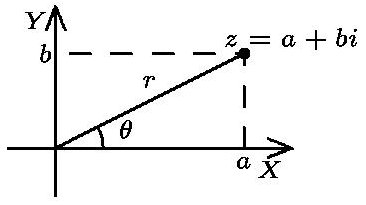
\includegraphics{complexgetal.jpg}
\item\textcolor{green}{\hypertarget{goniometrische_vorm}{Goniometrische vorm:}}\label{goniometrische_vorm}
		\[a+bi=r(\cos\theta +i\sin\theta)\]
\item\textcolor{green}{Product en quoti\"ent van twee complexe getallen:}\vskip 0.3 cm
Zij $z_1=r_1(\cos\theta_1 +i\sin\theta_1)$ en $z_2=r_2(\cos\theta_2+i\sin\theta_2)$.\vskip 0.3 cm Er geldt:
\[z_1\cdot z_2=r_1r_2(\cos(\theta_1+\theta_2)+i\sin(\theta_1+\theta_2)\] \vskip 0.3 cm
\[\ds\Frac{z_1}{z_2}=\ds\Frac{r_1}{r_2}(\cos(\theta_1-\theta_2)+i\sin(\theta_1-\theta_2)\]
\item\textcolor{green}{n-de macht van een complex getal:}\vskip 0.3 cm
\[\forall n\in \Z: (r(\cos\theta+i\sin\theta))^n=r^n(\cos n\theta + i\sin n\theta)\]\vskip 0.3 cm
\item\textcolor{green}{Formule van De Moivre:}
\[(\cos \theta +i\sin\theta)^n=\cos n\theta+i\sin n \theta\]\vskip 0.3 cm
\item\textcolor{green}{n-de machtswortels uit een complex getal $\:z=r(\cos\theta+i\sin\theta)$:}
\[\sqrt[n]{r}\cdot(\cos\ds\Frac{\theta+k\cdot 360^{\circ}}{n}+i\sin\ds\Frac{\theta+k\cdot360^{\circ}}{n})\: \mbox{met}\: k\in \Z\]
\end{itemize}\vskip 0.3 cm
\item \hypertarget{exponentiele_vorm}{{\bf Exponenti\"ele schrijfwijze van een complex getal $x+iy$}}\label{exponentiele_vorm}
\begin{itemize}%expon
\item \textcolor{green}{Formules}
\[x+iy=r e^{\theta i}=r(\cos\theta+i\sin\theta)\]
\[e^z=e^{x+iy}=e^x(\cos y+i\sin y)\]
\item \textcolor{green}{Gevolg}
\[\cos z =\ds\Frac{1}{2}(e^{zi}+e^{-zi})\]
\[\sin z =\ds\Frac{1}{2i}(e^{zi}-e^{-zi})\]
\end{itemize}%expon
\item \hypertarget{veeltermen_over_C}{{\bf Veeltermen over \C}}\label{veeltermen_over_C}
\begin{itemize}%veeltermen C
\item[*] Elke veelterm over $\C$ van de $n$-de graad heeft precies $n$ nulpunten in $\C$.
\item[*] Als het complexe getal $a+bi$ een nulpunt is van een veelterm met {\bf re\"ele} co\"effici\"enten, dan is ook het complex toegevoegde getal $a-bi$ een nulpunt van deze veelterm.
\end{itemize} %veeltermen C
\end{enumerate}%complexe getallen

\subsection{Statistiek} \label{statistiek}
\hypertarget{statistiek}{}
\begin{enumerate}%statistiek
\item\textcolor{green}{\hypertarget{begrippen}{Enkele begrippen:}}\label{begrippen}
\begin{itemize}% begrippen
\item {\it Populatie (universum)}: de verzameling van personen of objecten waarvan men 						kenmerk(en) wil onderzoeken
\item {\it Steekproef}: deelverzameling van de populatie, verzameling van die elementen van de 			populatie waarvoor de waarnemingen worden uitgevoerd.
\item {\it Variabele}: kenmerk dat men bij de elementen van de populatie wil nagaan. Aan de   				variabele worden waarden toegekend.  
\end{itemize}%begrippen
\item\textcolor{green}{\hypertarget{frequentietabel}{Frequentietabel:}}\label{frequentietabel}\newline
Stel $x_1, x_2, x_3, \ldots, x_n$ een steekproef met omvang $n$ en $p$ verschillende waarden.
\begin{center}
\begin{tabular}{|c|c|c|}
\hline
$x$ & absolute frequentie & relatieve frequentie\\ \hline
$x_1$ & $n_1$ & $f_1$ \\
$x_2$ & $n_2$ & $f_2$ \\
$\vdots$ & $ \vdots$ & $\vdots$\\
$x_p$ & $n_p$ & $f_p$ \\
\hline
\end{tabular}
\end{center}
\begin{itemize}
\item \hypertarget{absolute_frequentie}{{\bf Absolute frequentie:}}\label{absolute_frequentie} $n_i$ is het aantal keer dat de waarde $x_i$ voorkomt in de steekproef; er geldt:\vskip 0.5cm
\[\sum_{i=1}^{p}{n_i}=n\]
\item \hypertarget{relatieve_frequentie}{{\bf De relatieve frequentie:}}\label{relatieve_frequentie} $f_i=\ds\Frac{n_i}{n}$ en er geldt:
 \[\sum_{i=1}^{p}{f_i}=1\]
OF in procent: $f_i=\ds\Frac{n_i}{n}\cdot 100$ en er geldt:
\[\sum_{i=1}^{p}{f_i}=100\]
\end{itemize}
\item\textcolor{green}{\hypertarget{gemiddelde}{Gemiddelde($\bar{x}$):}}\label{gemiddelde}
\begin{itemize}
\item $\bar{x}=\Frac{1}{n}\sum_{i=1}^{p}{n_i\,x_i}$
\end{itemize}
Dit wordt ook wel {\it gewogen} gemiddelde genoemd.
\item\textcolor{green}{Variantie $(s^2)$ en \hypertarget{afwijking}{standaardafwijking $(s)$:}}\label{afwijking}
\begin{itemize}
\item $s^2=\ds\Frac{1}{n}\cdot\sum_{i=1}^{p}{n_i(x_i-\bar{x})^2}$
\item $s=\sqrt{\ds\Frac{1}{n}\cdot\sum_{i=1}^{p}{n_i(x_i-\bar{x})^2}}$
\end{itemize}
\end{enumerate}%statistiek


% Dit werk is gelicenseerd onder een Creative Commons
% Naamsvermelding-GelijkDelen 3.0 Unported.
% Bezoek http://creativecommons.org/licenses/by-sa/3.0/ om een kopie te zien 
% van de licentie of stuur een brief naar Creative Commons, 444 Castro Street, 
% Suite 900, Mountain View, California, 94041, USA.